\chapter{Combined ABCD Rules and Dermoscopic Structures using Bayesian Network}

\section{Introduction}
This chapter is about the development of the proposed CAD framework for automating ABCD rules (Asymmetry, Border, Colour, and Dermoscopic structures) using SVM models and Bayesian fusion.

\section{Related Work}
A paper described by Javier Lopez, et al.\cite{Lopez-Labraca2018} describes a CAD system designed to provide doctors with an enriched diagnosis. They utilise data extraction and classification techniques on dermoscopic structures, followed by combining the output of individual features using a bayesian approach. This provides an indication of which features are impact the diagnosis.




\subsection{Detection Algorithms}
Ihab S. zaqout\cite{Zaqout2016} describes a technique using the centroid and rotation fo the skin lesion using moments of inertia. The skin lesion is folded over vertically and horizontally subtracting the opposite halves. Pixels that cannot be subtracted are summed and compared with a threshold. If over the threshold the skin lesion is consdered asymmetrcial in that direction.

Reda Kasmi and Karim Mokrani\cite{Kasmi2016} describes a technique for comparing the colour distibution of the skin lesion by splitting the lesion into a 20x20 grid and comparing it against the colour of the perpendicular square using the 3D euclidean distance. If over a threshold that square is considered asymmetrical. If more than half the lesions are over the threshold then the area is considered asymmetrical.


\section{Discussion}
Automatic systems are being developed for the early detection of melanoma because it can take 10 years of experience for an accuracy of 86\%\cite{Morton1998}. Melanoma is one of the most aggressive forms of cancer that can remain dormant from anywhere between 6 months and 10 years before developing into metastatic melanoma, which becomes substially more difficult to cure\cite{UK2019}. Problematically, clinicians that are not trained specifically to diagnose melanoma are usually the first to attempt it. Improving the accuracy of these clincians should increase the overall accuracy of detecting melanoma. The early detection of melanoma followed by a biopsy is known to completely cure the disease\cite{}. Furthermore, melanoma develops from melancytes that create the skins pigmentation through the production of melanin, making a brown patch on the skin. Therefore, it has a clear indiciation of development on the surface of the skin. This means it is ideal for the creation of computer vision models for its early detection.

For these reasons there has been further interest in developing an automatic system for helping clinicians to detect melanoma at its early stages. However, regardless of newer systems being developed they are still rarely implemented within clincal environments. This is largely because of many systems producing what is called a parallel diagnosis, which do not provide an explanation on how results were reached\cite{Lipton2018}. These techniques usually utilise Convolutional Neural Netoworks (CNN) because of there superior accuracy\cite{Wen2022}. These are referred to as `black-box' approaches because while they provide a diagnosis there is often little to no explanations to the results its reached\cite{Andre2017}. There needs to be further explanations of the diagnosis for doctors to understand and properly utilise within clinical environments. 

Newer machine learning models utilise explainable AI (XAI) to provide an explanation which provides further insight\cite{skar2017}. While, these provide some indication on which area of the image has been used to train the agorithm they are still not tied directly to relevant clincal features. Furthermore there appears to be a tradeoff between interpretability and the models performance. Clinicans might not want to utilise models that are more interpretable, but less accurate. Furthermore, there has been some indication of models producing realistic but incorrect results\cite{Lipton2018}. In some scenarios clinicians might be misled to falsly diagnose a skin lesion. Due to the high stakes involved when diagnosing melanoma there needs to be highly accurate explanations and a track record of success before utilising them.

This chapter proposes a CAD framework for the detection of melanoma using data extraction techniques to ensure the use of relevent features. The aim is to produce a transparent system focusing on providing information that would be useful to dermatologists and the impact of those features on the diagnosis. Metadata is included regarding age, gender, anatomical location. Other features are asymmetry, border, colour, and dermoscopic structures. These are then combined using a Bayesian network. Case-based reasoning is also implemented to find skin lesions with similar clinical features.

\section{Detection of ABCD Rules}
%Briefly cover the techniques, tested and proven in previous chapter
ABCD rules in this chapter referres to the asymmetry, border, colour and dermoscopic structures. Sometimes the D in ABCD rules referes to the diameter of the skin lesion, but it is often removed for dermocopic structures because images are taken at different distances making the measurement of diameter unreliable. Furthermore, the detection of dermocopic structures provides valuable information in detecting the melanoma mimic called seborrhoeic keratosis (SK)\cite{Minagawa2017}. 

Asymmetry detection utilised 


\section{Proposed Framework}
The proposed CAD framework described in Figure\ref{model} automates the ABCD rules using statistical algorithms to extract features ($f$) from asymmetry, border, colour, and dermoscopic structures. Each feature has an associated SVM model trained using these extracted features. Next, Bayesian fusion, a probabilistic approach, combines multiple independent classifiers to diagnose melanoma. One benefit of Bayesian fusion is its higher accuracy in classifying skin lesions as compared to a standalone classifier\cite{Takruri2017}.  Javier López-Labraca, et al describe a similar method using dermoscopic structures, and colour\cite{Lopez-Labraca2018}. Other benefits are estimating the relevance of individual classifiers and classifying them with incomplete data, making it an interpretable and robust method. In addition, some feature extraction techniques generate graphics that might be suitable as an explanation for the diagnosis. Finally, the PH$^2$ dataset validates the rules, and once combined into a diagnosis, more extensive datasets, including ISIC 2019, measure its accuracy based on diagnosis.

\begin{figure}
\begin{tikzpicture}[]

	%Image Acqusition
	\node (inp) [img] at (0, 3) {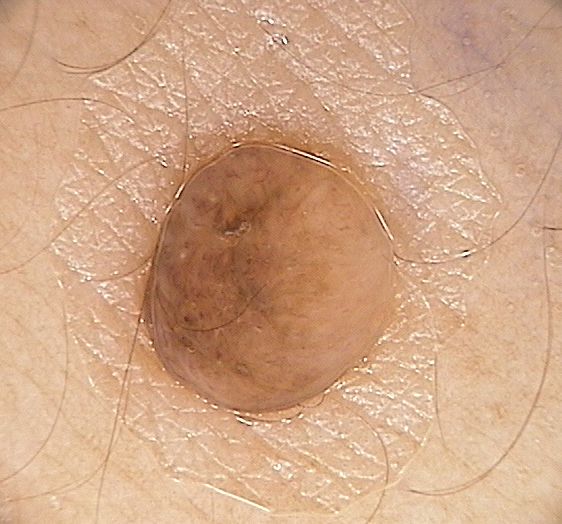
\includegraphics[scale=0.12]{lesion.png}};
	
	%Pre-processing
	\node (aug) [box, minimum height=1cm, node distance=3.6cm, right of=inp] {Augmentation};
	\node (seg) [box, minimum height=1cm, node distance=3.6cm, right of=aug] {Segmentation};
	
\node[draw=white] at ($(aug.north west)+(1.3,0.5)$) {\textbf{Pre-processing}};

\draw[thick, dotted] ($(aug.north west)+(-0.3,0.3)$) rectangle ($(seg.south east)+(0.3, -0.3)$);		

    %Feature extraction
    \node (asy) [box, right of=seg] at (0.0, 0.4) {Asymmetry};
    \node (bor) [box, right of=seg] at (0.0, -0.8) {Border};
    \node (col) [box, right of=seg] at (0.0, -2.0) {Colour};
    
    \node (asy2) [box, minimum width=1cm, right of=asy] {$f_a$};
	\node (bor2) [box, minimum width=1cm, right of=bor] {$f_b$};
    \node (col2) [box, minimum width=1cm, right of=col] {$f_c$};

		\node[draw=white] at ($(asy.north west)+(1.9,0.5)$) {\textbf{Feature Extraction}};    
    
    \draw[thick, dotted] ($(asy.north west)+(-0.3,0.3)$) rectangle ($(col2.south east)+(0.3, -0.3)$);
    
    %Classification
    \node (asy3) [box, right of=asy2] {SVM$_a$};
	\node (bor3) [box, right of=bor2] {SVM$_b$};
    \node (col3) [box, right of=col2] {SVM$_c$};

	\node[draw=white] at ($(asy3.north west)+(1.3,0.5)$) {\textbf{Classification}};    
    
    \node (fus) [box, minimum height=3cm, minimum width=1.7cm, text width=2cm] at (10.56, -0.8) {Bayesian \\ Fusion};
    
    \draw[thick, dotted] ($(asy3.north west)+(-0.3,0.3)$) rectangle ($(fus.south east)+(0.3, -0.3)$);
      
    \node (out) [box, right of=fus, node distance=2.7cm, minimum height=1.9cm, minimum width=1.9cm, text width=2cm] {Benign or \\ Malignant};
    
	\draw[->]
			(aug) edge (seg)
			(asy) edge (asy2)
			(bor) edge (bor2)  
			(col) edge (col2)  
			(asy2) edge (asy3)
			(bor2) edge (bor3)  
			(col2) edge (col3)  
			  
;
	\draw[->] (bor3)
	-|	($(fus.west)+(-0.5, 0)$)
 	|- (fus)
;

	\draw[-] (asy3)
	-|	($(bor3.east)+(0.5, 0)$)
;

	\draw[-] (col3)
	-| ($(fus.west)+(-0.5, 0)$)
;

 	\draw[->] (inp) edge (aug)
 			(asy2) edge (asy3)
			(bor2) edge (bor3)  
			(col2) edge (col3)  
 			(fus) edge (out)
 				(seg) -| ($(seg.east)+(0.7, 0)$)
 					  |- ($(seg.east)+(0, -1.2)$)
 					  -| ($(asy.west)+(-0.8, 0)$)
 					  |- (asy)
;

 	\draw[->] ($(asy.west)+(-0.8, 0)$) 
 		  |- (bor)
;

	\draw[->] ($(asy.west)+(-0.8, -1.2)$) 
 		  |- (col)
; 
    
\end{tikzpicture}
\caption{Proposed CAD framework describing the segmentation, feature extraction  and classification process.}\label{model}
\end{figure}

ABCD rules describe the classification process for each rule and demonstrate the process behind reaching diagnoses. The objective is to visualise important features that GPs might need to support their diagnostic procedure. Hopefully, this will instantiate trust when automating skin lesion identification within clinical environments. Another advantage would be the automatic labelling of skin lesions, making it easier for dermatologists to identify later.

The CAD framework in figure\ref{model} describes a model of pre-processing, feature extraction, and classification stages. After segmentation, statistical algorithms extract features ($f$), representing a different rule. Next, SVM models individually process the extracted features and combine them into a final result between benign and malignant using Bayesian fusion.

